\chapter{Notification \& Commentaires}
\section{Introduction}
\paragraph{}
Dans une autre phase d'implémentation de la plateforme, comme dans les autres réseaux sociaux il est indispensable de notifier l'utilisateur dans le cas du partage d'un stample, une catégorie, le demande d'ajout, ect...
\subparagraph{}
Stample offre la possibiliter d'organiser le contenu diffusé sur la plateforme sous forme des catégories, le partage de ces derniers c'est une nouvelle fonctionnalité qu'on trouve sur dropbox, sauf que pour Stample les catégories sont organisées sous forme d'une arborescence similaire à un système de fichier.
\newline
Le stample ou dit autrement l'article c'est un contenu qui peut être écrit en précisant le titre, le contenu, l'auteur, la source, ect...
Peut être aussi générer par des darg \& drop en utilisant le clipper depuis un autre site.
\subparagraph{}
Ces options avec le partage des stample, nécessitent de notifier les utilisateurs de la plateforme en option avec l'email et sous forme d'une alert sur le site.
\newline
Les commentaires présentent aussi une fonctionnalité intéressante pour interragir avec le contenu d'un stample.
\section{Notifications}
\paragraph{}
La figure 5.1 présente le design et les différentes étapes du getNotifications.
\begin{figure}[H]
        \centering
                \centering
                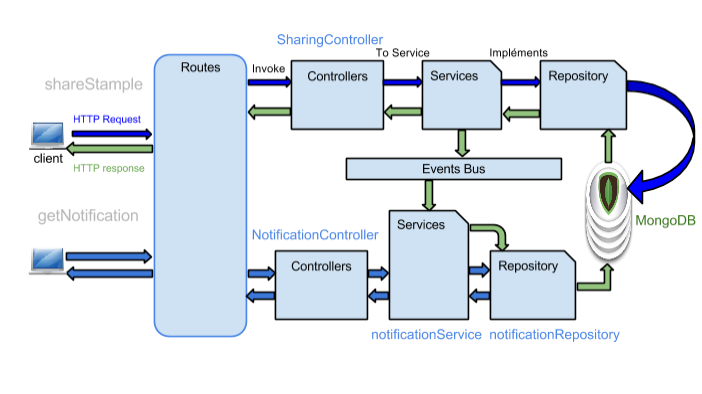
\includegraphics[width=\textwidth]{Notifications.png}
               \caption{getNotifications design}
		\label{fig:getNotifications design}
\end{figure}
\subsection{Système de Notifications}
Les notifications sont représentées dans la base de données par une collection "notification\_inbox" identifier par un "\_id" ObjectID et des "notifications" sous forme d'une liste d'objet Notification(content, id, date, isRead) intialiser à "Null".
On utilise un modéle de notification "deux cases classes"(NotificationInbox, Notification).
Les notifications sont gérées dans la base de données grâce à des fontions (getNotificationsForUser, addNotification, deleteNotification, ect ...).
On utilise ces méthodes implémentées dans "Notification repository" pour nos services (getNotification, deleteNotification, ect...).
Les différentes routes utilisées pour les notifications font appel au "notificationController" pour le "get, read, delete" Notifications.
\subsection{Problèmes}
Après l'implémentation des services de notifications, nous avons eu un problème de sécurité au niveau de l'envoie des informations utilisateurs avec les notifications "l'objet JSON" retourné.
\subparagraph{}
Pour résoudre ce problème nous avons défini un filtre "simpleFilterProvider" dans lequel on ajoute un "Set" des données privées. Cela permet de d'enlever tous les informations inutiles dans "l'objet JSON".


\section{Tests d'intégration des commentaires}
\paragraph{}
Dans cette partie, j'ai travaillé sur l'implémentation des tests d'intégrations et des services update, delete comment.
\begin{figure}[H]
        \centering
                \centering
                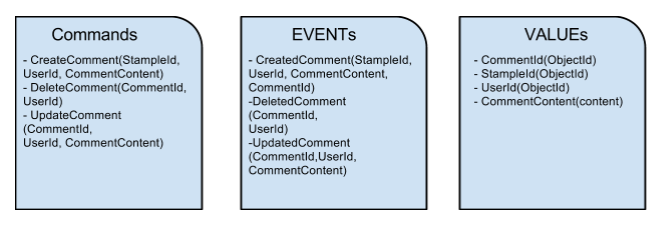
\includegraphics[width=\textwidth]{Comment.png}
               \caption{Architecture des comments}
		\label{fig:Design des commentaires}
\end{figure}
\subparagraph{}
Etapes d'intégration :
\begin{enumerate}
\item La création des "events" pour les différentes "case classes" utilisées dans les APIs.
\item L'ajout des values des "case classes" pour identifier les Comments, Stamples, Users. 
\item L'implémentation des services.
\end{enumerate}
\subparagraph{}
Les tests unitaires, d'intégration sont écrits en Specs2 (software specification for Scala) : C'est une librairie pour écrire des spécifications des softwares executables. Le lancement des test se fait via sbt sur la console.
Vous trouverez par suite deux captures d'écran une pour le lancement du test sbt et l'autre du code.
Il faut ajouter les dependencies du plugin dans le fichier ApplicationBuilt du projet.
\newpage
\subparagraph{}
Vous trouverez ci-dessous deux imprimes écran des tests d'intégration pour les commentaires ainsi que vous pouvez voir le succè des tests sur le terminal.
\begin{figure}[H]
        \centering
                \centering
                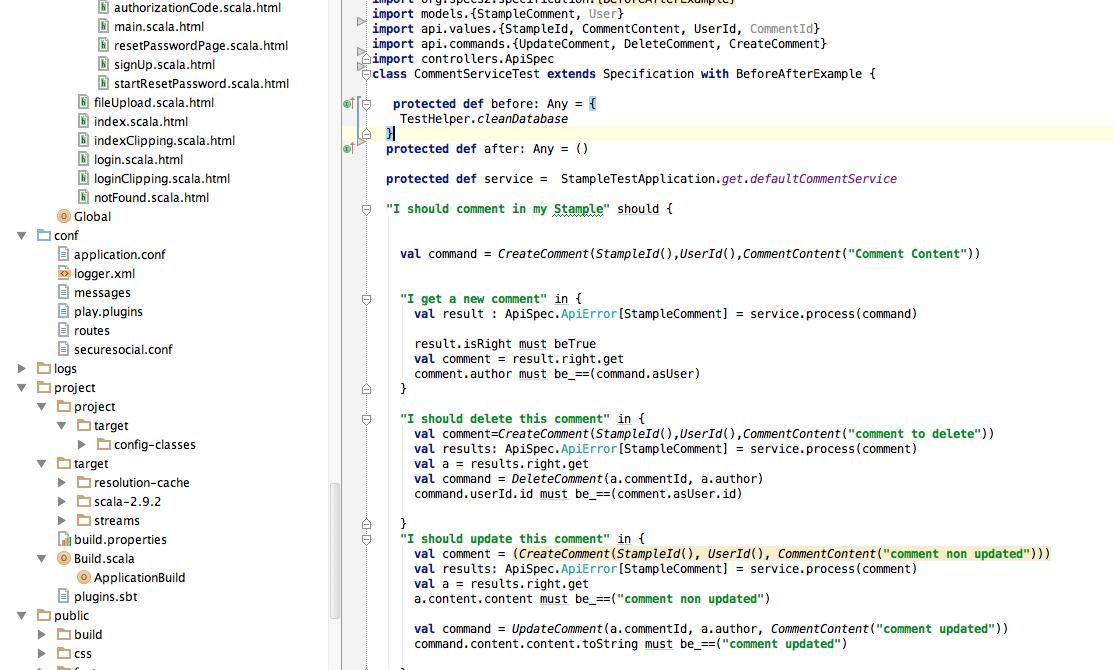
\includegraphics[width=\textwidth]{test.png}
               \caption{Tests Code}
		\label{fig:Test Code}
\end{figure}
\begin{figure}[H]
        \centering
                \centering
                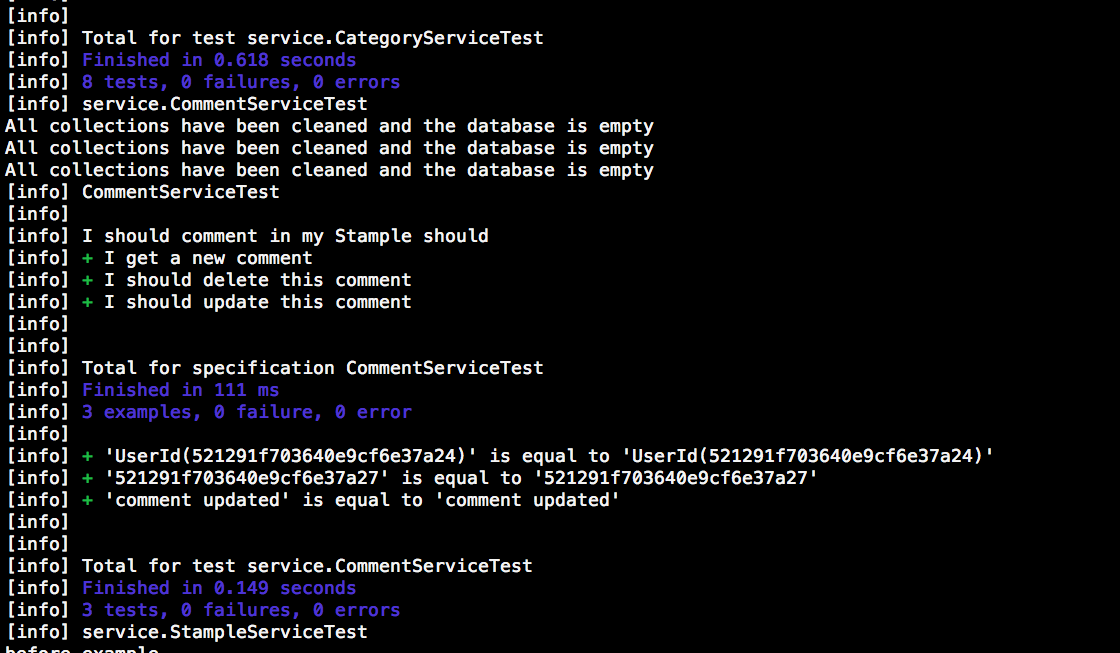
\includegraphics[width=\textwidth]{code.png}
               \caption{Tests Code}
		\label{fig:Test Code}
\end{figure}
\section{Résumé}
\paragraph{}
Dans cette partie du Stage, j'ai découvet le systéme de notification en travaillant sur des sous tâches, une première approche pour le commentStample et j'ai écris les tests nécessaires pour la création, la mise à jour et la suppression des commentaires.
\subparagraph{}
Le chapitre suivant présentera une étude sur des altérnatives relative un futur Stample en cours de construction.
Des bibliothéques sont mises en ligne un projet open source "banana-rdf" et "RWW-Play", Henry Story et des membres du W3C, travaillent sur ces bibliothéques.